%\section{La structure des quasicristaux}
%%Each section needs a subsection for the small points on top to show up
%\subsection{Dummy}
%\begin{frame}{Quasicrystals}
%Aperiodic yet ``ordered'' arrangement of atoms/molecules/colloids
%
%A quasicrystal has the following properties:
%\begin{itemize}
%	\item it is \textbf{aperiodic}
%	\item it is \textbf{long range ordered} (its diffraction pattern exhibits sharp peaks).
%\end{itemize}
%%\textbf{Aperiodic tilings} are used to model quasicrystals.
%\(
%	\<{6cm}
%		\centering
%		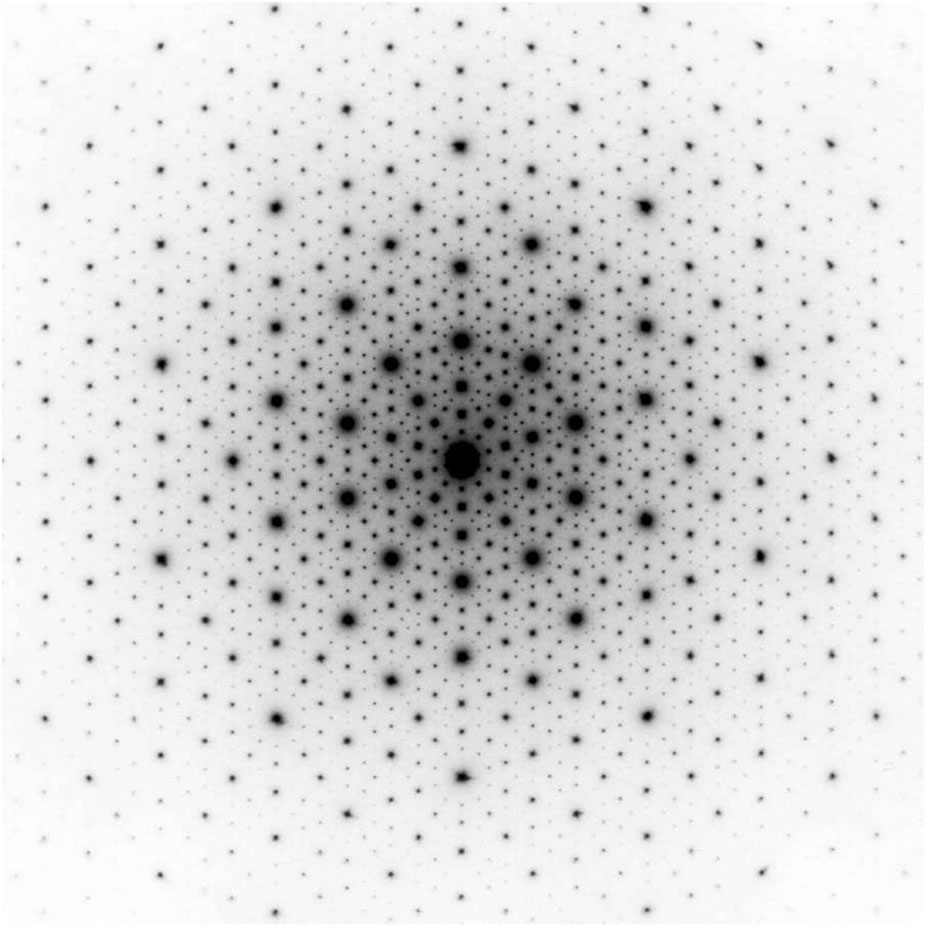
\includegraphics[scale=0.1]{img/1_intro/diffraction_tenfold.png}
%		
%		\ss{Figure de diffraction d'un alliage d'AlPdMn} \ss{(groupe de Conradin Beeli)}
%	\>
%	\<{6cm}
%		\centering
%		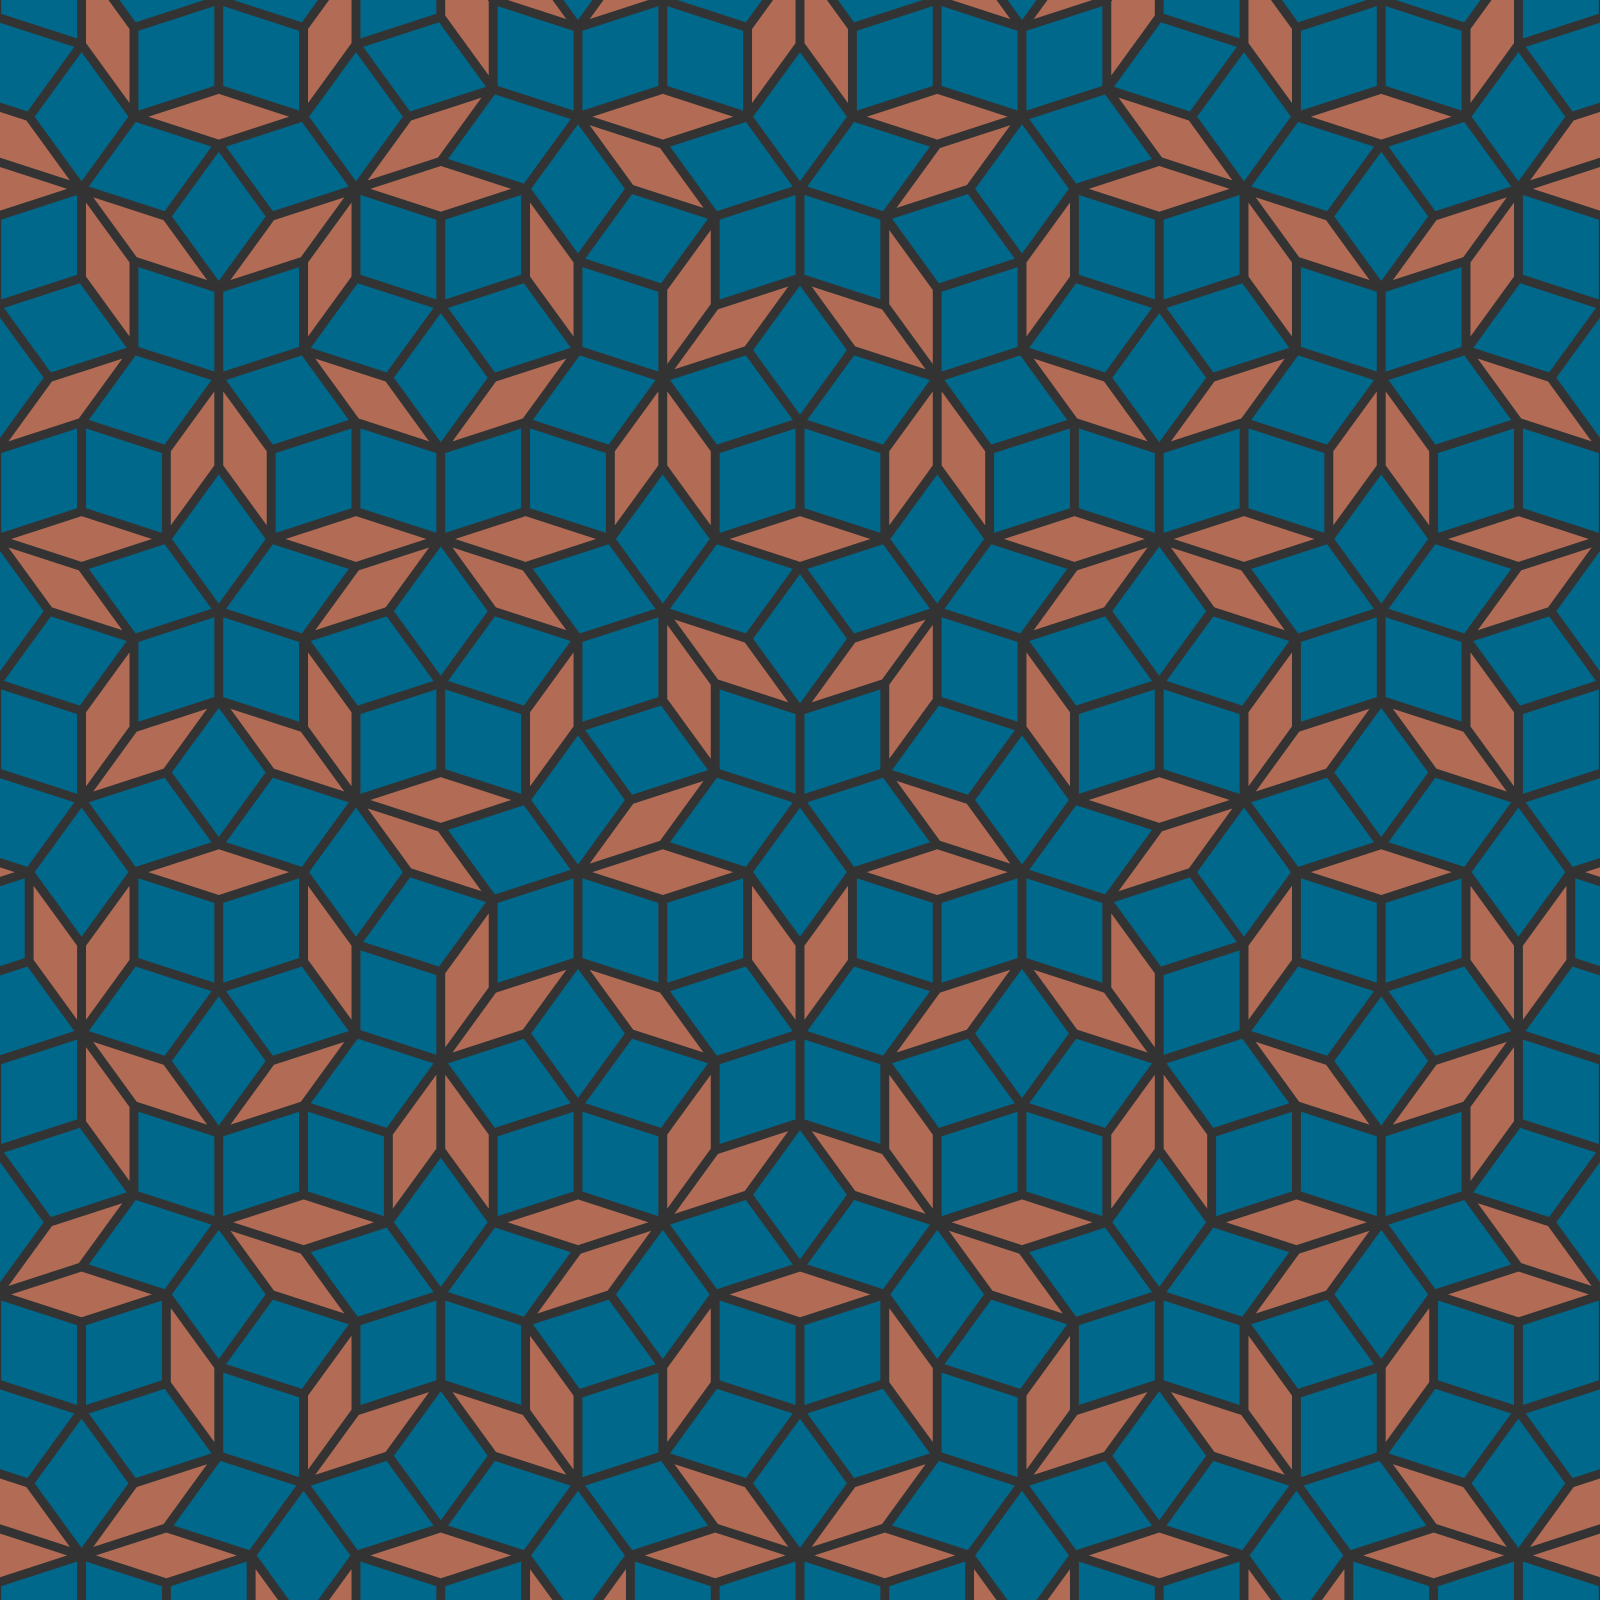
\includegraphics[scale=0.06]{img/1_intro/penrose.png}
%		
%		\ss{Un morceau du pavage de Penrose,} \ss{souvent utilisé pour modéliser les quasis.}
%	\>
%\)
%\end{frame}
%
%\begin{frame}{Exemples de quasicristaux}
%\(
%	\<{6cm}
%		\centering
%		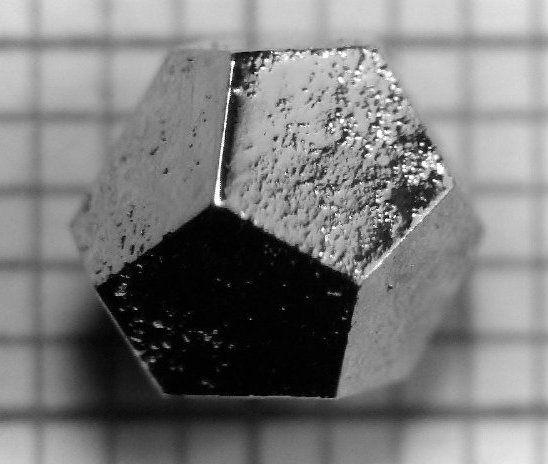
\includegraphics[scale=0.28]{img/1_intro/homgzn.png}
%		
%		\ss{HoMgZn alloy in its icosahedral phase} \ss{(\url{doi:10.1038/nmat1244})}
%	\>
%	\<{6cm}
%		\centering
%		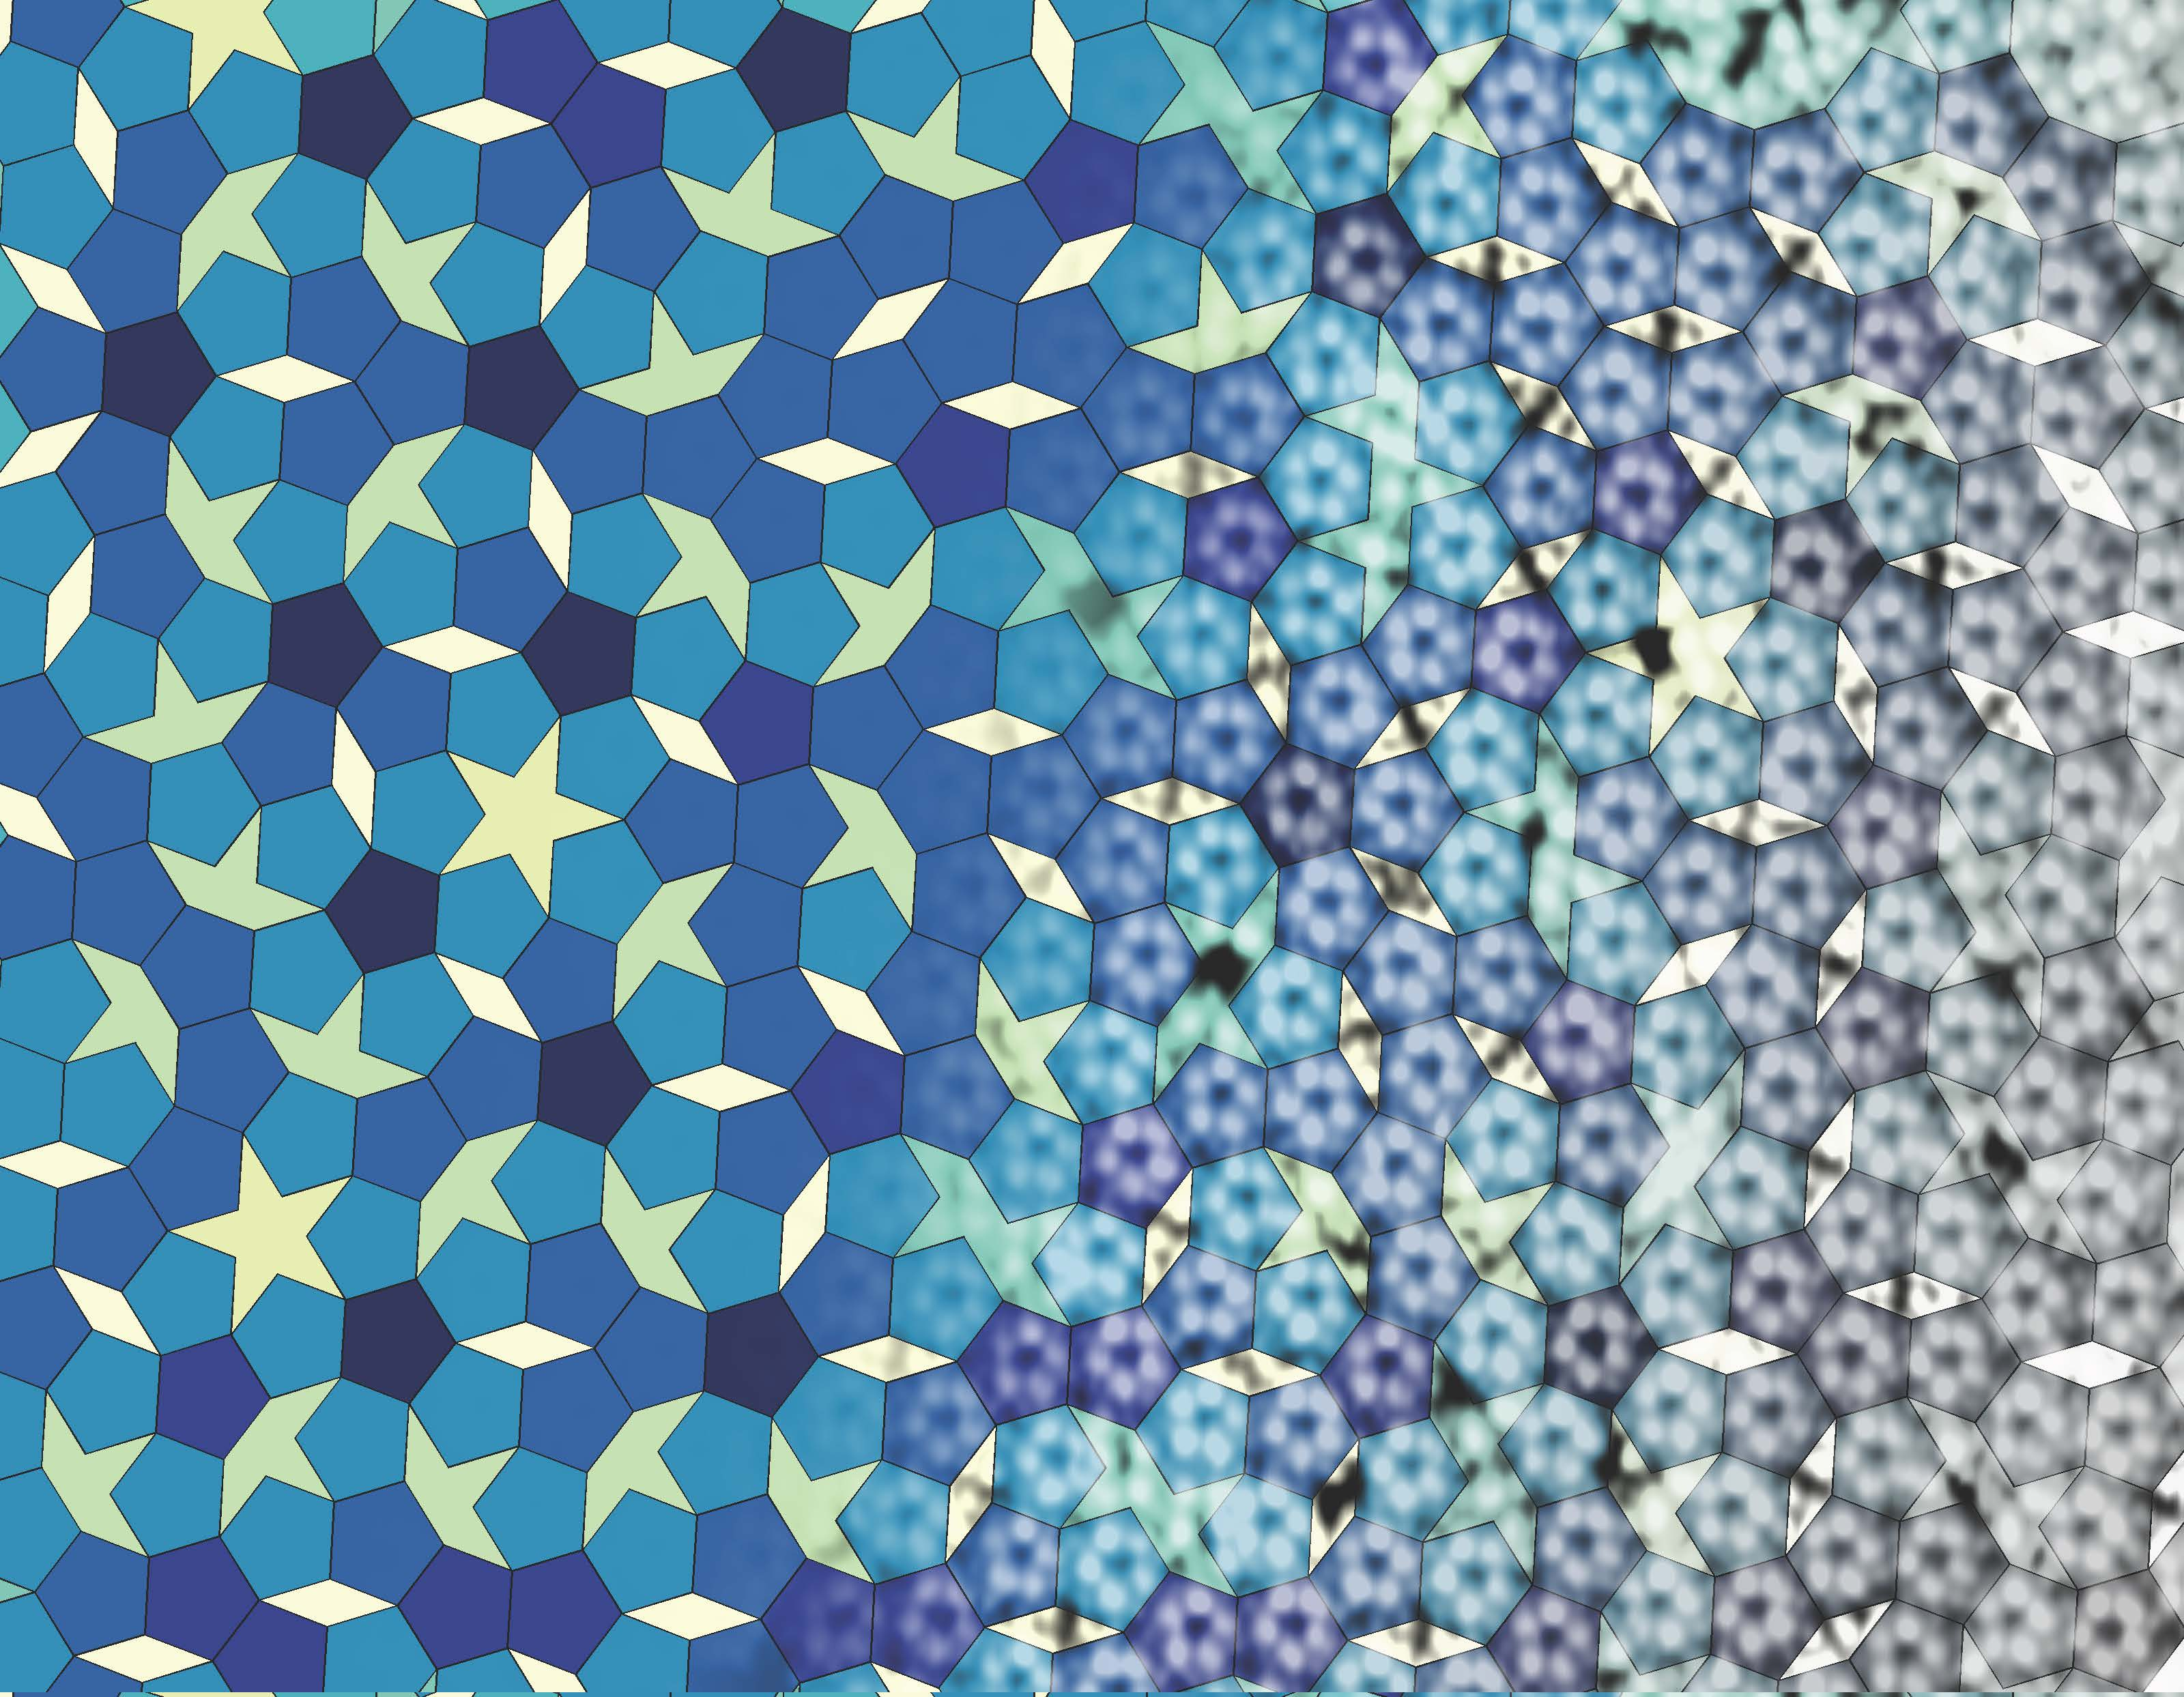
\includegraphics[scale=0.22]{img/1_intro/wasio.jpg}
%		
%		\ss{A 2D molecular quasicrystal} \ss{(\url{doi:10.1038/nature12993})}
%	\>
%\)
%
%\begin{itemize}
%	\item many intermetallic alloys are quasiperiodic
%	\item a single natural example: Khatyrka meteorite hosts quasicrystals \ss{(\url{doi:10.1126/science.1170827})}. 
%\end{itemize}
%\end{frame}

\begin{frame}{A puzzle [Bédaride \etal{} 12]}

\centering
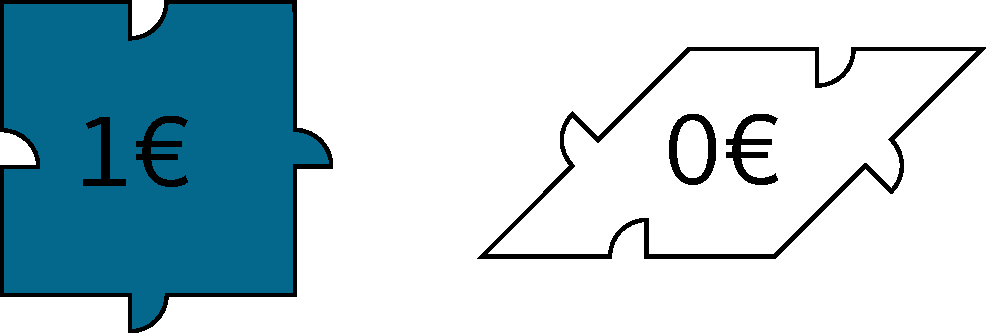
\includegraphics[width=.5\textwidth]{img/1_intro/tiles_euro.pdf}

Pay the squares, get the rhombuses for free!

\(
\<{6cm}
\centering
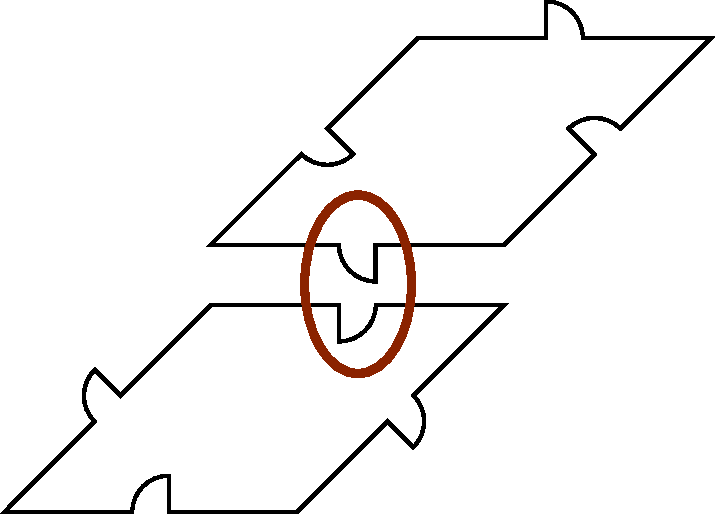
\includegraphics[width=.8\textwidth]{img/1_intro/forbidden.pdf}

Forbidden configuration.
\>

\<{6cm}
\centering
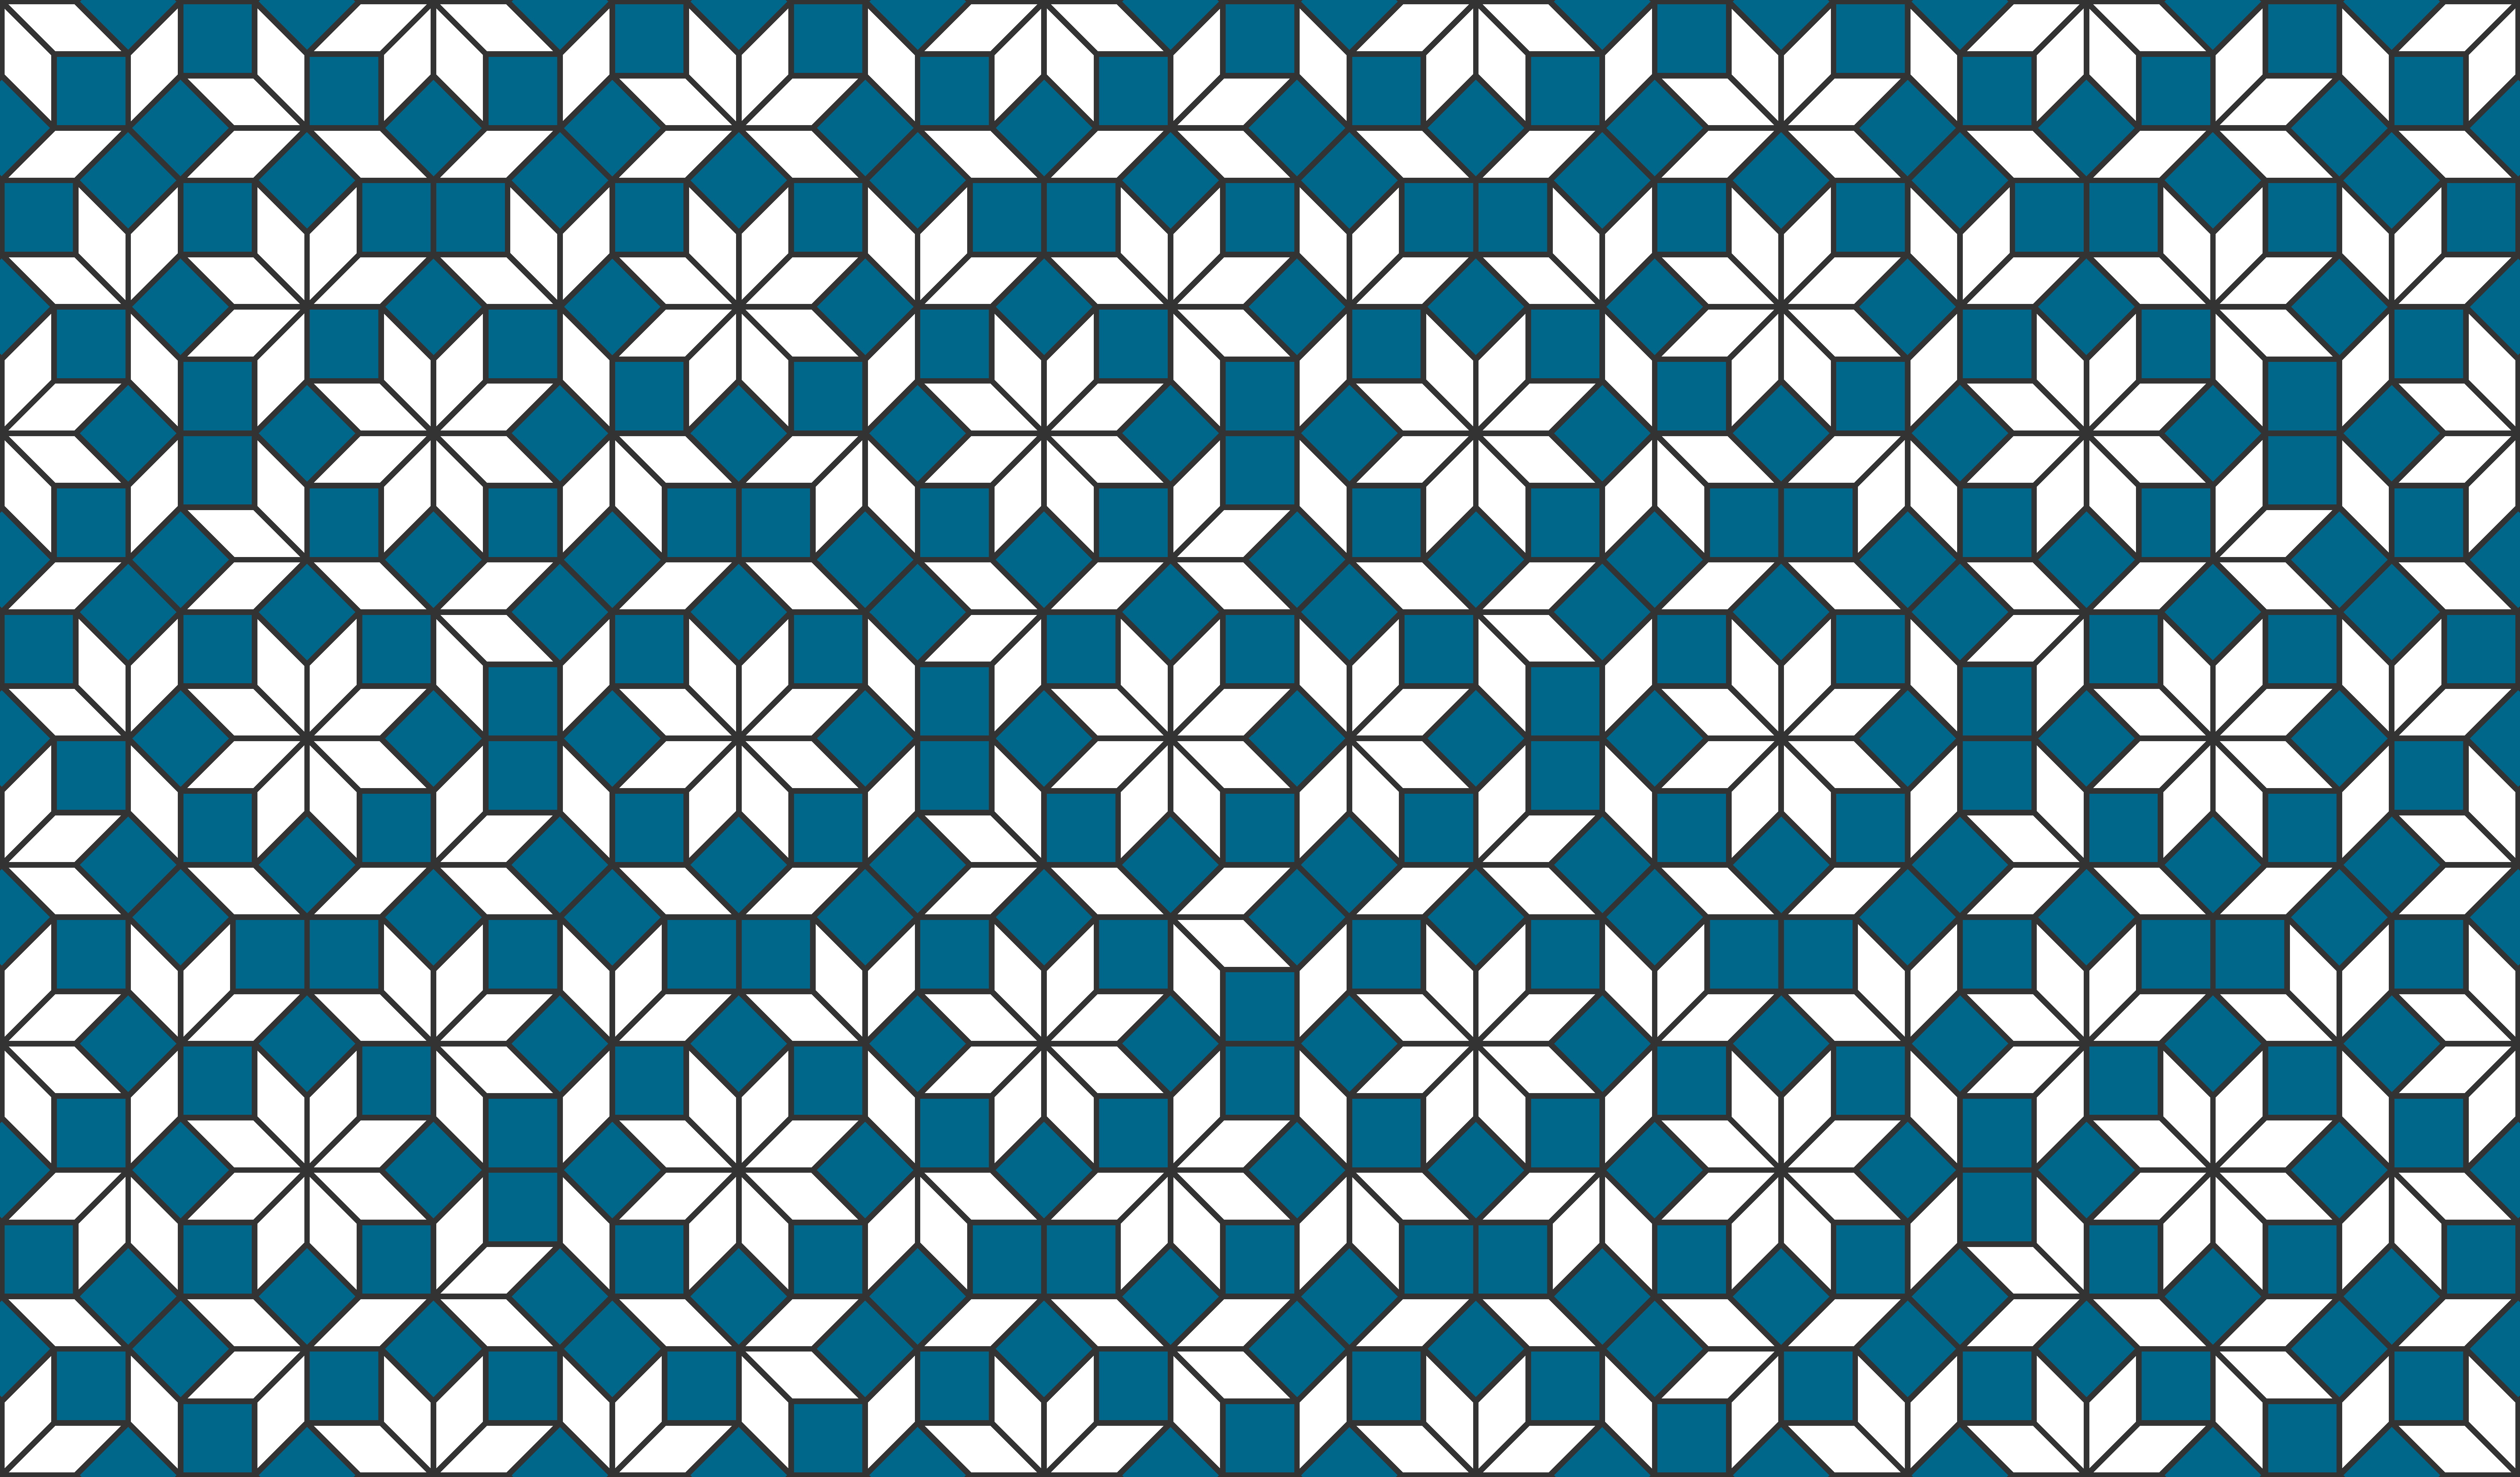
\includegraphics[width=1.\textwidth]{img/1_intro/ammann.pdf}

Patch of the Ammann-Beenker tiling.
\>
\)

\end{frame}